\documentclass[a4paper,12pt]{article}
\usepackage[russian]{babel} % (нельзя с polyglossia)
\usepackage{fontspec}
\setmainfont[Ligatures=TeX]{Times New Roman} % Шрифт для основного текста
\setsansfont[Ligatures=TeX]{Arial}
\setmonofont{Consolas} % Шрифт для кода
\usepackage{amsmath, amssymb} % Для математических формул
\usepackage[left=1.45cm, right=1.45cm, top=1.5cm, bottom=1.5cm]{geometry} % Настройка полей
% \usepackage{pdflscape} % Поворот страниц в PDF
\usepackage{graphicx}

\usepackage{yfonts} % - доп. готические символы
\usepackage{pifont} % доп. символы

\usepackage{bm}

\usepackage{xcolor}
\usepackage{enumitem}
\usepackage{ulem}
\usepackage{tcolorbox}

\usepackage{booktabs}

\AtBeginDocument{\boldmath} % Опционально: все мат.элементы жирным шрифтом

\usepackage{adjustbox}

\usepackage{float} % Для жесткой фиксации изображений [H]

\setlength{\parindent}{0pt} % Опционально: отрубаем по рофлу красную строку

\usepackage[colorlinks=true]{hyperref}
\hypersetup{
	colorlinks=true,
	linkcolor=blue, % Почему-то зависит от colorlinks=true
}

%-------------------РУССКАЯ НУМЕРАЦИЯ В ENUMERATE-------------------%
% Создаем команду для русских букв
\newcommand{\rusitem}[1]{
	\par % без этого почему-то первый пункт оставался на строке с текстом
	\stepcounter{ruscount}
	\noindent
	\ifcase\value{ruscount}\or а)\or б)\or в)\or г)\or д)\or е)\or ж)\or з)\or и)\or й)\or
	к)\or л)\or м)\or н)\or о)\or п)\or р)\or с)\or т)\or у)\or
	ф)\or х)\or ц)\or ч)\or ш)\or щ)\or ъ)\or ы)\or ь)\or э)\or ю)\or я)\fi
	\ #1\par
}

% Создаем новый счетчик
\newcounter{ruscount}

%-------------------ЦВЕТНОЙ ФОН ФЛОМАСТЕРА-------------------%
% Цвета
\definecolor{lightblue}{RGB}{202,244,255}
\definecolor{pink}{RGB}{255,230,245}

% Цветные боксы
\newtcolorbox{highlightbox}{
	colback=lightblue,
	colframe=lightblue,
	boxrule=0pt,
	arc=3mm,
	auto outer arc,
	boxsep=2mm,
	left=2mm, right=2mm, top=1mm, bottom=1mm
}

\newtcolorbox{pinkbox}{
	colback=pink,
	colframe=pink,
	boxrule=0pt,
	arc=2mm,
	auto outer arc,
	boxsep=1mm,
	left=1mm, right=1mm, top=0.5mm, bottom=0.5mm
}

%-------------------КРУГОВАЯ ОБВОДКА-------------------%
\usepackage{titlesec}
\usepackage{tikz}

% Универсальная команда для обводки
\newcommand{\circled}[1]{
	\tikz[baseline=(char.base)]{
		\node[draw,circle,inner sep=1pt,minimum size=1.2em](char){\strut #1};
	}
}

% Модифицированная команда для разделов с обведённым номером
\newcommand{\circledsection}[2][]{
	% \refstepcounter{section} % Раскомментировав - раздел будет считаться в общей нумерации
	\par\vspace{4ex plus 1ex minus .2ex}
	\noindent{\Large\bfseries\circled{\thesection}~#2\par} % \thesection передает номер из оглавление в раздел
	\addcontentsline{toc}{section}{\protect\numberline{\thesection}#2} % С #1 будет убрано название и останутся только точки
	\vspace{2.5ex plus .2ex}
}

% Модифицированная команда для подразделов с обведённым номером
\newcommand{\circledsubsection}[1]{
	\refstepcounter{subsection} % Отвечает за нуммерацию
	\par\vspace{3.25ex plus 1ex minus .2ex}
	\noindent{\large\bfseries\circled{\thesubsection}~#1\par}
	\addcontentsline{toc}{subsection}{\protect\numberline{\thesubsection}#1}
	\vspace{2.3ex plus .2ex}
}

% Стандартные подразделы (если раскомментить - subsection* (без нумерации) перестанет работать)
% \makeatletter
% \renewcommand{\subsection}{\@startsection{subsection}{2}{\z@}
%	{-3.25ex\@plus -1ex \@minus -.2ex}
%	{1.5ex \@plus .2ex}
%	{\normalfont\large\bfseries}
% }
% \makeatother

% Реализация списков со сквозной нумерацией (просто \item в них писать не надо)
\newcounter{flexcounter}
\newlist{flexlist}{enumerate}{3}
\setlist[flexlist]{
	before=\setcounter{flexcounter}{0},
	label={\arabic*.},
	ref=\arabic*,
	align=left,
	leftmargin=*,
	labelwidth=!,
	labelindent=0pt
}

\newcommand{\flexlabel}[1]{
	\ifnum\value{flexcounter}>0\relax
	\arabic{flexcounter}.
	\fi
}

\newcommand{\circleditem}{
	\refstepcounter{flexcounter}
	\item[\circled{\arabic{flexcounter}}]
}

\newcommand{\plainitem}{
	\refstepcounter{flexcounter}
	\item[\arabic{flexcounter}]
}

%-------------------ДЕЛАЕМ ТОЧКИ ОГЛАВЛЕНИЯ АКТИВНЫМИ-------------------%
% Переопределяем \@dottedtocline для полной ссылки
\makeatletter
\def\@dottedtocline#1#2#3#4#5{
	\ifnum #1>\c@tocdepth \else
	\vskip \z@ \@plus.2pt
	{\leftskip #2\relax
		\rightskip \@tocrmarg \parfillskip -\rightskip
		\parindent #2\relax\@afterindenttrue
		\interlinepenalty\@M
		\leavevmode
		\@tempdima #3\relax
		\begingroup
		\ifnum #1=1 \bfseries \fi % Жирный шрифт только для первого уровня
		\parindent \z@ \leftskip #3\relax
		% \advance\leftskip by 1.5em % - задаем сдвиг подзаголовка
		% \hskip -\leftskip % - двигаем подзаголовок влево
		\hyper@linkstart{link}{\Hy@tocdestname}
		#4 % текст заголовка
		\leaders\hbox{$\m@th
			\mkern \@dotsep mu\hbox{.}\mkern \@dotsep mu$}\hfill
		\nobreak\hb@xt@\@pnumwidth{\hfil #5} % номер страницы
		\hyper@linkend
		\endgroup
		\par}
	\fi}
% Переопределяем \l@section для использования \@dottedtocline
\renewcommand*\l@section[2]{
	\ifnum \c@tocdepth >\z@
	\addpenalty\@secpenalty
	\addvspace{1.0em \@plus\p@}
	\@dottedtocline{1}{0em}{1.5em}{#1}{#2}
	\fi}
\makeatother


\begin{document}
	
	\tableofcontents
	\newpage
	
	\section{Зависимости структурные, по данным и управлению. Способы преодоления зависимостей. Построение статической и динамической трассы исполнения команд.}
	\vspace{-1em}
	\subsection{Общая информация}
	\vspace{-0.5em}
	\textbf{Конвейеризация} -- это разбиение выполняемой функции на последовательные этапы (ступени), каждой из которых соответствует отдельный аппаратный блок.
	
	\vspace{-1em}
	\begin{figure}[H]
		\centering
		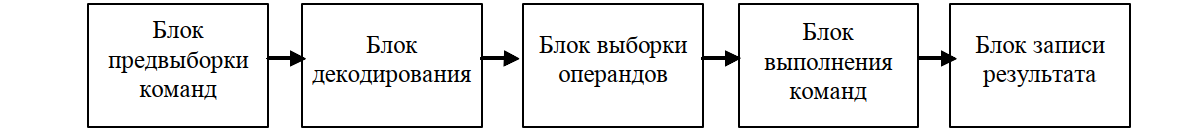
\includegraphics[width=1\linewidth, height=0.075\textheight]{img/01_01}
		\par
		{\small Разбиение процессора на блоки выполнения команд}
		\label{fig:01_01}
	\end{figure}
	\vspace{-1em}
	
	Команды проходят через эти блоки по тактам, при этом на разных ступенях одновременно обрабатываются разные команды. Если каждый этап занимает один такт, процессор выдает результат новой команды каждый такт. Такая организация значительно повышает производительность и широко используется в современных высокопроизводительных процессорах.
	\par\vspace{0.5em}
	\textbf{Конвейеризация} -- способ обеспечения параллельности выполнения команд.
	
	\textbf{Суперконвейер} -- это обычный конвейер, разбитый на более мелкие этапы. Он позволяет увеличить тактовую частоту процессора, но его длина ограничена рядом факторов. Основные ограничения связаны с зависимостями между командами, которые могут замедлять их продвижение по конвейеру.
	
	\par\vspace{0.5em}
	
	В зависимости от типа команды, вида способа адресации время выполнения 
	команды сильно варьируется. Дольше всего выполняются этапы, связанные с 
	обращением к памяти.
	
	\vspace{-1em}
	\begin{figure}[H]
		\centering
		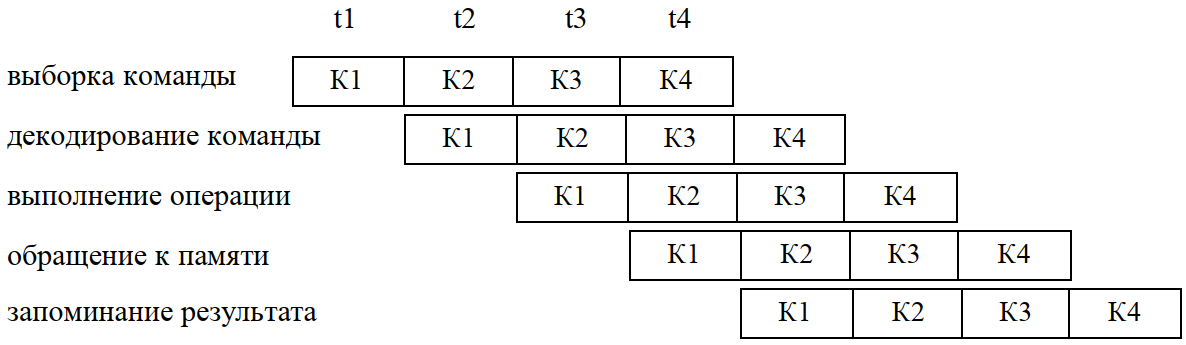
\includegraphics[width=1\linewidth, height=0.175\textheight]{img/01_02}
		\par
		{\small Работа конвейера}
		\label{fig:01_02}
	\end{figure}
	\vspace{-1em}
	
	Конвейеризация повышает пропускную способность процессора (число команд, завершаемых за единицу времени), но не сокращает время выполнения одной команды. 
	\par 
	Эффективность ограничивается накладными расходами, связанными с несбалансированными задержками на ступенях: тактовая частота определяется самой медленной из них.
	
	\par\vspace{0.5em}
	\textbf{Поток команд} -- естественная последовательность команд, проходящая по конвейеру процессора. 
	\par
	Современные суперпроцессоры могут обрабатывать несколько потоков, если для каждого этапа предусмотрены отдельные исполнительные элементы.
	\par\vspace{0.5em}
	
	Максимальная эффективность достигается при высокой загрузке конвейера и равномерной подаче команд и данных (типично для RISC-процессоров). Задержки снижают производительность, особенно при возникновении \textbf{конфликтов}, которые делятся на три типа:
	
	\begin{enumerate}
		\item \textbf{Структурные} -- нехватка аппаратных ресурсов для одновременного выполнения команд.
		\item \textbf{По данным} -- одна команда зависит от результата предыдущей.
		\item \textbf{По управлению} -- связаны с переходами и изменением счётчика команд.
	\end{enumerate}
	
	При конфликтах конвейер частично останавливается: приостановка одной команды блокирует последующие, а новые команды не загружаются, что увеличивает среднее время выполнения.
	
	\newpage
	
	\subsection{Структурные зависимости}
	
	Появляются из-за недостаточности ресурсов. 
	\par 
	\textbf{\uline{Пример}}: наличие единственного конвейера доступа к памяти как для команд, так и для данных. 
	\par
	Это приводит к конфликту, если:
	\vspace{-0.35em}
	\begin{itemize}
		\item одна команда обращается к памяти за данными,
		\item в то же время происходит выборка следующей команды из памяти.
	\end{itemize}
	\vspace{-0.5em}
	\textbf{\uline{Решение}}:
	\vspace{-0.35em}
	\begin{itemize}
		\item приостановка конвейера на один такт -- \textbf{вставка конвейерного пузыря (pipeline bubble)}.
	\end{itemize}
	\vspace{-1.5em}
	\subsection{Зависимости по данным}
	
	Связаны с использованием одних и тех же ресурсов (регистров, ячеек памяти) в разных инструкциях.
	
	\textbf{\uline{Классификация зависимостей по данным:}}
	
	\begin{itemize}
		\item \textbf{RAW (Read After Write)} – чтение после записи (\textit{наиболее общий и важный тип конфликтов}). 
		\par
		Инструкция пытается прочитать значение до того, как предыдущая завершит запись. 
		\par
		\item \textbf{WAR (Write After Read)} – запись после чтения. 
		\par
		Инструкция записывает значение раньше, чем другая инструкция успела его прочитать.
		\item \textbf{WAW (Write After Write)} – запись после записи. 
		\par
		Две инструкции записывают в один и тот же регистр, но порядок записи нарушен.
		\item \textbf{RAR (Read After Read)} – чтение после чтения. 
		\par
		Не приводит к конфликтам и может быть проигнорировано.
	\end{itemize}
	
	\textbf{\uline{Типичная ситуация}}:

	\begin{itemize}
		\item Команда B использует результат команды A, но команда A еще не завершила выполнение.
		\item Если продолжить выполнение без доп. мер, B может использовать некорректные данные.
	\end{itemize}
	
	\textbf{\uline{Методы разрешения конфликтов}}:
	
	\begin{enumerate}
		\item \textbf{Обходы (data bypassing) / закоротки (short-circuiting)}
			\begin{itemize}
				\item Результат выхода АЛУ возвращается напрямую на его вход, т.е. выбирается значение, 
				\par
				идущее по цепи обхода, минуя регистровый файл.
				\item Применимо к случаям RAW-зависимости между двумя операциями АЛУ.
			\end{itemize}
		\item \textbf{Внутренние блокировки (pipeline interlock)}:
		\begin{itemize}
			\item Используется в случае, когда обход невозможен
			\par
			\textbf{\uline{Пр.}:} после команды \texttt{LW} (имеет задержку и не может быть решена обычной ``пересылкой'').
			\item Аппаратура автоматически приостанавливает выполнение последующих инструкций.
			\item Возникает ``пузырь'' в конвейере.
		\end{itemize}
	\end{enumerate}
	Сейчас компиляторы применяют планирование команд для повышения эффективности конвейера.
	\par
	\textbf{Базовый блок} -- линейная последовательность без переходов. Позволяет минимизировать простои. 
	\par
	В простом случае команды упорядочиваются внутри базового блока с учётом графа зависимостей.
	\par
	Планирование упрощается, т.к. выполнение блока команд зависит от выполнения первой команды.
	\newpage
	Однако, требуются более сложные алгоритмы планирования. Они базируются на следующих методах:
	\begin{enumerate}[start=3]
		\item \textbf{Динамическая оптимизация (``out-of-order execution'' - неупорядоченное выполнение)}:
		\begin{itemize}
			\item Буферизация конфликтующих команд.
			\item Продолжение выполнения других независимых инструкций в ``обход'' буфера.
			\item Передача результата в зависимую команду или на вход устройства, минуя запись в регистр.
		\end{itemize}
		\item \textbf{Переименование регистров (register renaming)}:
		\begin{itemize}
			\item Используются логические и физические регистры.
			\item Логические регистры отображаются на физические с помощью таблиц отображения.
			\item Каждый новый результат сохраняется в новый физический регистр.
			\item Предыдущее значение сохраняется для возможного отката.
			\item Временные значения фиксируются после завершения команды.
			\item Устраняются зависимости WAW и WAR.
			\item Программист работает только с логическими регистрами.
			\item Позволяет избежать конфликтов за один и тот же логический регистр.
		\end{itemize}
	\end{enumerate}
	
	\subsection{Зависимости по управлению}
	
	Возникают из-за наличия условных переходов в программе. 
	\par
	\textbf{\uline{Пример}}:
	
	\begin{itemize}
		\item Выполнение команды B зависит от результата команды A.
	\end{itemize}
	
	\textbf{\uline{Причины}}:
	
	\begin{itemize}
		\item Управляющие конструкции: \texttt{if}, \texttt{while}, \texttt{for}.
	\end{itemize}
	
	\textbf{\uline{Методы снижения влияния}}:
	
	\begin{itemize}
		\item \textbf{Реорганизация кода} -- минимизация зависимостей.
		\item \textbf{Асинхронные операции} -- продолжение выполнения без ожидания.
		\item \textbf{Кэширование} -- повторное использование результатов операций.
	\end{itemize}
	
	\textbf{Существуют два вида переходов}:
	
	\begin{enumerate}
		\item \textbf{Безусловные} -- всегда выполняются.
		\item \textbf{Условные} -- выполняются в зависимости от результата сравнения.
	\end{enumerate}
	
	\textbf{\uline{Проблема}}: Нельзя заранее узнать, выполнится ли условный переход, до окончания его выполнения. 
	\par
	Чтобы не терять такты при ожидании прохождения команды исполнительной ступени конвейера, используется предсказание. При верном -- выполнение продолжается, при ошибке -- конвейер очищается и перезапускается с нужного адреса.
	\par
	Есть простые способы уменьшить задержки конвейера, вызванные условными переходами:
	
	\textbf{\uline{Решения}}:
	
	\begin{enumerate}[leftmargin=2em]
		\item \textbf{Метод выжидания} -- заморозка конвейера до определения направления перехода путем \uline{блокировки} выполнения любой команды за командой условного перехода до определения его направления.
		\item \textbf{Метод возврата (предсказание как \uline{невыполняемого})} -- продолжение исполнения, как будто переход не произойдет. Состояние машины \uline{не изменяется} до определения направления перехода.
		\item \textbf{Задержанные переходы (delayed branch)} -- выполнение перехода \uline{с задержкой}, в течение которой исполняются другие команды. Эти команды находятся в слотах (временных интервалах) задержанного перехода.
	\end{enumerate}
	
	\newpage
	
	\subsection{Методы предсказания переходов}
	
	\subsubsection{Статическое предсказание (static prediction)}
	
	Осуществляется в основном \uline{до выполнения программы}:
	
	\begin{itemize}[leftmargin=2.25em]
		\item \textbf{На этапе компиляции}:
		\begin{itemize}[leftmargin=1.35em]
			\item Метод \uline{исследования структуры} программы (её анализ).
			\item Метод \uline{использования профиля выполнения} программы (\uline{трассировка} предыдущих запусков).
			\par
			$\bullet$ Компилятор устанавливает флаг, указывающий направление перехода.
		\end{itemize}
		\item \textbf{На этапе выполнения}:
		\begin{itemize}[leftmargin=1.35em]
			\item Применение заранее заданных правил (пример: предположение, что переход назад -- цикл).
		\end{itemize}
	\end{itemize}
	
	\subsubsection{Динамическое предсказание (dynamic prediction)}
	
	Происходит во время исполнения программы и основано на анализе истории ветвлений.
	
	\begin{enumerate}[leftmargin=1.35em]
		\item \textbf{Метод прогнозирования условных переходов}
		\par
		Используется \textbf{буфер предсказания (таблица ``истории'') условных переходов}:
		\begin{itemize}
			\item Небольшая память (таблица), индексируемая по младшим битам адреса команды перехода.
			\item Каждая ячейка содержит бит, указывающий, был ли предыдущий переход выполнен.
			\item \uline{Однобитовая схема} -- прогноз меняется сразу при ошибке, что плохо для циклов.
			\item \uline{Двухбитовая схема} -- прогноз меняется только после двух ошибок, что повышает точность.
			\item Возможны более сложные n-битовые и коррелированные схемы, учитывающие историю нескольких переходов.
		\end{itemize}
		
		\item \textbf{Метод быстрого определения адреса перехода}
		\par
		Используется \textbf{буфер целевых адресов переходов (branch target buffer)}:
		\begin{itemize}
			\item Кэш хранит адреса следующих команд для переходов.
			\item Позволяет быстро определять адрес следующей команды и сокращать задержки.
			\item Используется вместе \uline{с буфером предсказания} для мгновенного выбора ветви.
		\end{itemize}
		
		\item \textbf{Метод свертывания переходов (branch folding)}
		\par
		Используется \textbf{буфер целевых адресов переходов (branch target buffer)}:
		\begin{itemize}
			\item Хранит команды из прогнозируемой ветви внутри процессора.
			\item Позволяет уменьшить время выполнения безусловных и некоторых условных переходов.
			\item Может работать и самостоятельно -- \uline{без буфера целевых адресов}.
		\end{itemize}
		
		\item \textbf{Метод прогнозирования косвенных переходов}
		\par
		Используется \textbf{небольшой буфер адресов возврата, работающий как стек}:
		\begin{itemize}
			\item Косвенные переходы меняют адрес назначения во время выполнения -- в run-time 
			\par
			(например, возвраты из процедур).
			\item Буфер хранит последние адреса возврата и \uline{точно прогнозирует} следующий адрес.
		\end{itemize}
	\end{enumerate}
	
	\newpage
	
	\subsection{Трассы исполнения команд}
	
	\subsubsection{Статическая трасса исполнения}
	
	Создаётся на основе анализа исходного кода \uline{без его фактического выполнения}.
	
	\textbf{Используется для:}
	
	\begin{itemize}
		\item Оптимизации кода.
		\item Выявления потенциальных проблем.
	\end{itemize}
	
	\textbf{Включает:}
	
	\begin{itemize}
		\item Анализ потока управления.
		\item Анализ зависимостей данных.
	\end{itemize}
	
	\textbf{Пример:}
	\begin{itemize}
		\item Определяются места использования переменных и порядок исполнения инструкций.
	\end{itemize}
	
	\subsubsection{Динамическая трасса исполнения}
	
	Формируется \uline{во время выполнения} программы.
	
	\textbf{Используется для:}
	
	\begin{itemize}
		\item Профилирования.
		\item Отладки.
	\end{itemize}
	
	\textbf{Включает:}
	\begin{itemize}
		\item Последовательность реально выполненных инструкций.
		\item Фактические зависимости и данные, участвующие в исполнении.
	\end{itemize}
	
	\textbf{Пример:}
	\begin{itemize}
		\item Регистрируются команды, порядок их выполнения и используемые данные.
	\end{itemize}
	
	\textbf{Сравнение трасс позволяет:}
	\begin{itemize}
		\item Сравнение статической и динамической трасс позволяет выявить отклонения фактического выполнения от ожидаемого поведения, что помогает в отладке и оптимизации кода.
	\end{itemize}
	
	\textbf{Понимание типов зависимостей и методов их устранения позволяет:}
	\begin{itemize}
		\item Повысить производительность конвейерной архитектуры.
		\item Эффективно использовать ресурсы процессора.
		\item Оптимизировать исполняемый код на этапах компиляции и исполнения.
	\end{itemize}
	
	\newpage
	
	\section{Схемы основных мультипроцессорных архитектур (UMA, NUMA, векторная, сетевая, кластерная). Гранулярность. Классификация Флинна.}
	
	\subsection{Общая информация}
	% Введение в основные идеи
	$\bullet$ \textbf{ВМ} - вычислительная машина
	\par
	$\bullet$ \textbf{ВС} - вычислительная система
	\par
	Отличительная особенность ВС -- наличие средств параллельной обработки за счет построения параллельных ветвей в вычислениях, не предусмотренной классической структурой ВМ.
	\newline
	\textbf{Факторы эволюции архитектуры:}
	\begin{itemize}
		\item Требование увеличения вычислительной мощности для повышения производительности ВС.
		\item Переход от фон-неймановской архитектуры к параллельным вычислениям и многопроцессорным системам.
	\end{itemize}
	
	$\bullet$ \textbf{Топология} -- организация внутренних коммуникаций вычислительной системы.
	\newline
	$\bullet$ \textbf{Масштабируемость} -- способность системы эффективно расширяться за счёт увеличения числа процессоров, объёма оперативной и внешней памяти, а также других ресурсов.
	
	% Уровни параллелизма
	\subsection{Уровни параллелизма}
	\begin{itemize}
		\item \textbf{Уровень заданий}: независимые задания выполняются на разных процессорах одновременно.
		\par
		Этот уровень реализуется на ВС с множеством процессоров в многозадачном режиме. 
		\item \textbf{Уровень программ}: части одной задачи распределяются между процессорами.
		\par
		Данный уровень достигается на параллельных ВС.
		\item \textbf{Уровень команд}: команды исполняются параллельно или конвейерно.
		\par
		Уровень достижим на ВС с одним процессором.
		\item \textbf{Уровень битов}: обработка битов слова -- параллельная или последовательная.
		\par
		Данный уровень реализуется в обычных и суперскалярных процессорах. 
	\end{itemize}
	
	% Гранулярность с пояснениями
	\subsection{Гранулярность}
	Гранулярность -- это мера, отражающая соотношение объёма вычислений к объёму коммуникаций в параллельной задаче. Она тесно связана с уровнем параллелизма.
	\begin{itemize}
		\item \textbf{Крупнозернистый}: независимые программы (тысячи команд), редкий обмен данными.
		\par
		Этот уровень параллелизма обеспечивается операционной системой. 
		\item \textbf{Среднезернистый}: процедуры (сотни команд), управление программистом или компилятором.
		\par
		Обычно организуется как программистом, так и компилятором. 
		\item \textbf{Мелкозернистый}: небольшие вычисления (десятки команд), частый обмен данными.
		\par
		Этот уровень используется распараллеливающим (векторизирующим) компилятором.
	\end{itemize}
	
	Эффективное параллельное исполнение требует баланса м/у гранулярностью программ и коммуникационными задержками. В частности, в слабосвязанных задачах предпочтительно крупнозернистое разбиение.
	
	\newpage
	
	% Закон Амдала и формула
	\subsection{Закон Амдала}
	\begin{itemize}
		\item Ускорение зависит от числа процессоров и доли распараллеливаемой части программы.
		\item Формула ускорения \( S = \frac{T_{\text{однопроцессорной ВС}}}{T_{\text{параллельной ВС}}} \)
		\par
		Пусть программа имеет последовательную (f) и потенциально распараллеливаемую 
		части (1-f), тогда:
		\par
		\item Коэффициент ускорения \( S = \frac{1}{(1 - f) + \frac{f}{p}} \), где \( f \) -- параллельная часть, \( p \) -- число процессоров.
	\end{itemize}
	
	\vspace{-1.35em}
	\begin{figure}[H]
		\centering
		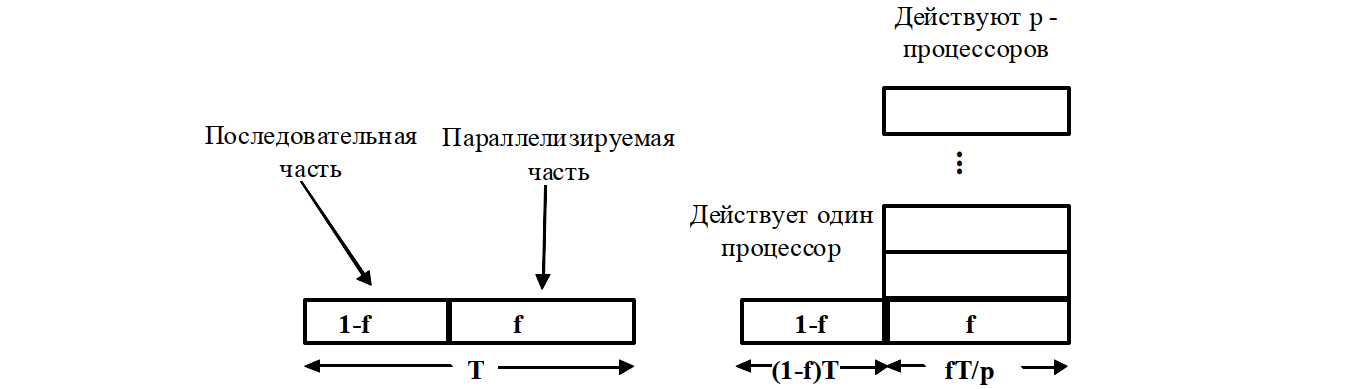
\includegraphics[width=1\linewidth, height=0.19\textheight]{img/02_01}
		{\small Разбиения программы на части}
		\label{fig:02_01}
	\end{figure}
	\vspace{-1em}
	Ниже приведенные графики иллюстрируют ускорение в зависимости от 
	количества параллельно работающих процессоров и процента распараллеливания кода.
	\vspace{-2em}
	\begin{figure}[H]
		\centering
		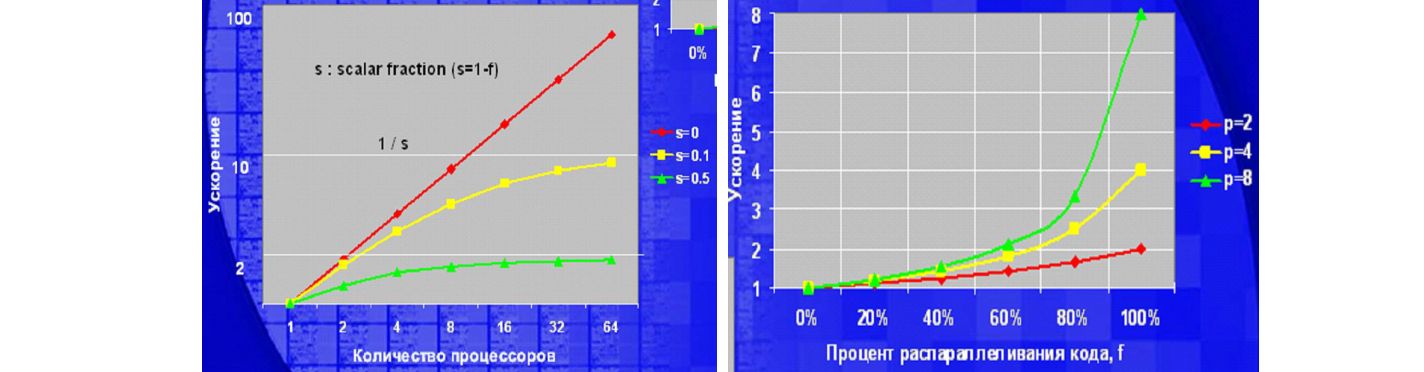
\includegraphics[width=1\linewidth, height=0.15\textheight]{img/02_02}
		{\small Ускорение за счет параллельного выполнения}
		\label{fig:02_02}
	\end{figure}
	\vspace{-1.25em}
	Существуют также и другие факторы, ограничивающие ускорение, к ним можно отнести:
	\begin{enumerate}
		\item \textbf{Программные издержки.} Параллельные алгоритмы, даже при тех же вычислениях, что и у последовательных, требуют дополнительных действий: индексных операций, учёта данных и распределения по процессорам -- всего того, что отсутствует в последовательных алгоритмах.
		\item \textbf{Издержки из-за дисбаланса загрузки процессоров.} При неравномерной нагрузке процессоры простаивают, ожидая других, что ограничивает ускорение самым медленным из них.
		\item \textbf{Коммуникационные издержки.} Обмен данными между процессорами снижает ускорение.
		\newline
		Для его уменьшения нужно крупнозернистое разбиение с минимальной долей коммуникаций.
	\end{enumerate}
	Также существует \textbf{закон Густафсона}, связывающий ускорение с числом процессоров.
	\vspace{-1em}
	
	% Информационные модели
	\subsection{Информационные модели}
	В параллельных системах обмен данными между процессорами зависит от гранулярности задач и осуществляется по одной из двух схем:
	\begin{itemize}
		\item \textbf{Память совместного использования}: единое адресное пространство для всех процессоров.
		\item \textbf{Распределенная память}: отдельные пространства, обмен через сообщения.
	\end{itemize}
	
	\textbf{Адресные модели:}
	\begin{itemize}
		\item \textbf{Общее адресное пространство}: процессоры обращаются к любой ячейке памяти.
		\item \textbf{Раздельные адресные пространства}: каждый процессор -- отдельный узел.
	\end{itemize}
	
	\newpage
	
	\textbf{Плюсы передачи сообщений:}
	\begin{itemize}
		\item Хорошая масштабируемость.
		\item Отсутствие потактовой синхронизации.
		\item Используются в наиболее производительных суперкомпьютерах.
	\end{itemize}
	
	\textbf{Минусы передачи сообщений:}
	\begin{enumerate}
		\item Более медленный и сложный обмен данными.
		\item Ограниченный объём локальной памяти.
		\item Высокая сложность и стоимость разработки ПО.
	\end{enumerate}
	
	% Классификация Флинна
	\subsection{Классы параллельных архитектур (Флинн)}
	\begin{itemize}
		\item \textbf{SISD}: один поток команд и данных -- классические машины.
		\item \textbf{SIMD}: один поток команд, много данных -- \textbf{потоковые} (векторные и матричные) процессоры.
		\item \textbf{MISD}: много команд, один поток данных -- конвейеры, но не все согласны.
		\item \textbf{MIMD}: много потоков команд и данных -- мультипроцессоры и мультикомпьютеры 
		\newline
		(деление предложено Э. Таненбаумом).
	\end{itemize}
	\vspace{-1.5em}
	\begin{figure}[H]
		\centering
		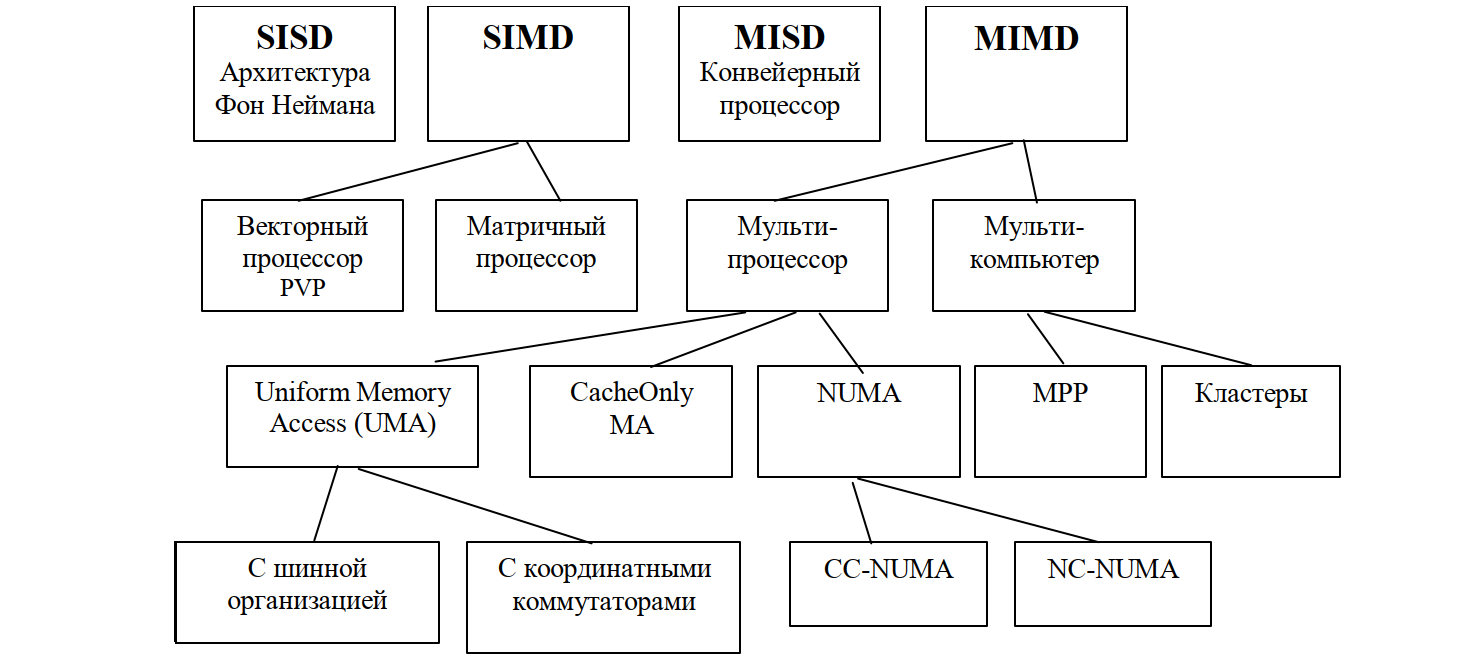
\includegraphics[width=1\linewidth, height=0.3\textheight]{img/02_03}
		{\small Расширенная классификация Флинна}
		\label{fig:02_03}
	\end{figure}
	\vspace{-2em}
	\begin{figure}[H]
		\centering
		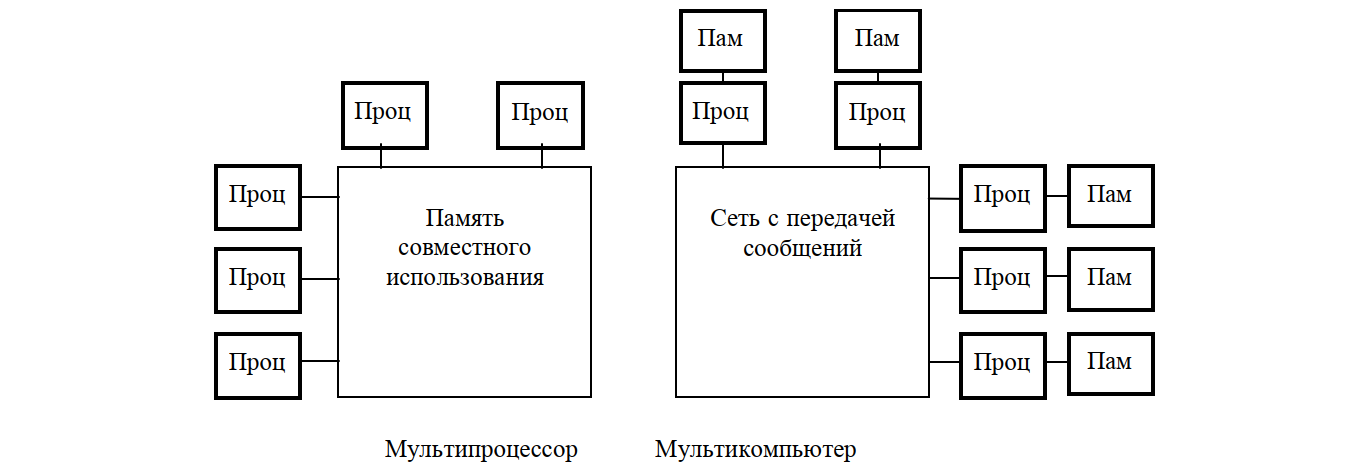
\includegraphics[width=1\linewidth, height=0.2\textheight]{img/02_04}
		{\small Информационные модели работы с памятью}
		\label{fig:02_04}
	\end{figure}
	
	\newpage
	
	Мультипроцессоры различают по доступу к памяти:
	\begin{itemize}
		\item \textbf{UMA} -- равное время доступа ко всем модулям памяти.
		\item \textbf{NUMA} -- доступ к локальной памяти быстрее, чем к удалённой.
		\item \textbf{COMA} -- отсутствует общая память, обмен через кеши.
	\end{itemize}
	
	Мультикомпьютеры делятся на:
	\begin{itemize}[leftmargin=1.5em]
		\item \textbf{MPP} -- дорогие суперкомпьютеры с множеством процессоров, соединённые высокоскоростной сетью.
		\item \textbf{Кластеры} -- недорогие системы из стандартных ПК, объединённых Ethernet или коммутатором. 
		\newline
		\uline {Гетерогенные (однородные)} -- объединены компьютеры разной мощности и разной архитектуры. 
		\newline
		Производительность зависит больше от сети, чем от процессоров.
    \end{itemize}
	
	\subsubsection{MPP архитектура (Massively Parallel Processing)}
	\begin{itemize}
		\item Массивно-параллельная система с большим числом процессоров.
		\item Каждый процессор имеет собственную память (разделённая память).
		\item Соединение через высокоскоростные коммуникационные каналы.
	\end{itemize}

	\subsubsection{SMP архитектура (Symmetric Multiprocessing)}
	\begin{itemize}
		\item Симметричная система с общей памятью и равным доступом процессоров.
		\item Высокоскоростная шина соединяет процессоры, память и ввод-вывод.
	\end{itemize}
	
	\subsubsection{FRC архитектура (Functional Redundancy Checking)}
	\begin{itemize}
		\item Пара master/checker процессоров для повышения надежности.
		\item Checker сравнивает результаты, не управляя шиной.
	\end{itemize}
	
	\subsubsection{PVP архитектура (Parallel Vector Process)}
	\begin{itemize}
		\item Векторно-конвейерные процессоры для параллельной обработки данных.
		\item Работают с общей памятью, как в SMP.
	\end{itemize}
	
	\subsubsection{Ассоциативные процессоры}
	\begin{itemize}
		\item Обработка по содержанию данных (SIMD-класс).
		\item Используют ассоциативные запоминающие устройства (АЗУ).
	\end{itemize}
	
	\newpage
	
	\subsection{Мультипроцессоры UMA с шинной организацией}
	\vspace{-0.5em}
	Архитектура UMA с шинной организацией -- простейшая форма мультипроцессорных систем,
	\newline
	использующая общую шину для равного доступа к физической памяти для всех процессоров.
	\begin{itemize}
		\item Используются дешевые и высокопроизводительные микропроцессоры.
		\item Ограничение производительности при числе процессоров более 16–32 из-за пропускной 
		\newline
		способности шины.
		\item Кэш-память в каждом процессоре уменьшает обращения к общей памяти.
	\end{itemize}
	\uline{Проблема}: кэширование разделяемых данных вызывает \uline{когерентность} кэш-памяти.
	\vspace{-1em}
	\begin{figure}[H]
		\centering
		\begin{minipage}[t]{0.49\textwidth}
			\centering
			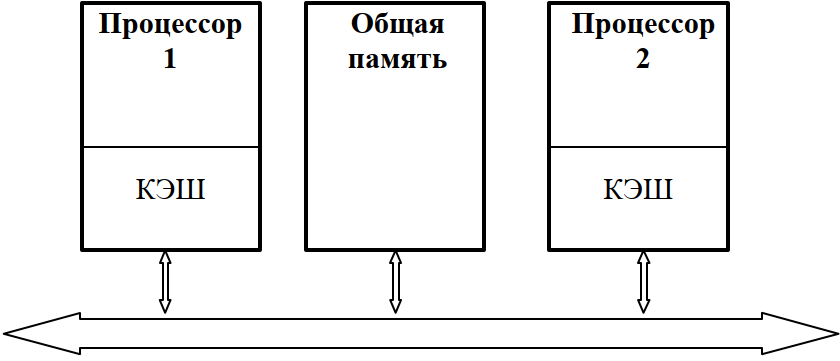
\includegraphics[width=\linewidth,height=3.3cm,keepaspectratio=false]{img/02_05}
			{\small Архитектура UMA с шинной организацией}
			\label{fig:02_05}
		\end{minipage}
		\hfill
		\begin{minipage}[t]{0.49\textwidth}
			\centering
			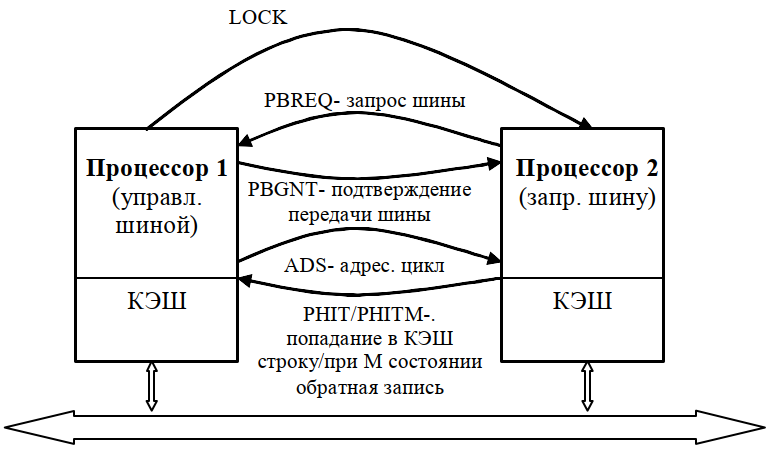
\includegraphics[width=\linewidth,height=4.6cm,keepaspectratio=false]{img/02_06}
			{\small Сигналы процессора Pentium}
			\label{fig:02_06}
		\end{minipage}
		\vspace{-1.5em}
	\end{figure}
	
	\subsubsection{Мультипроцессорная когерентность кэш-памяти}
	Проблема когерентности возникает из-за копий данных в кэшах разных процессоров.
	\begin{itemize}
		\item Решается с помощью аппаратных протоколов.
		\item Стратегия основана на смене состояний (например, MESI).
		\item Чтение возвращает последнее записанное значение при достаточном временном разрыве.
	\end{itemize}
	\vspace{-1em}
	\subsubsection{Протоколы поддержания когерентности данных}
	Протоколы обеспечивают согласованность данных в кэшах.
	\begin{itemize}
		\item Сквозная запись: запись в кэш дублируется в общую память, нагружая шину.
		\item Протоколы наблюдения: контроллеры кэшей следят за шиной, обновляя или аннулируя данные.
		\item Запись с аннулированием: аннулируются копии в других кэшах при записи.
		\item Запись с обновлением: копии в других кэшах обновляются при записи.
	\end{itemize}
	
	Имеются и другие менее распространенные протоколы:
	\begin{itemize}
		\item Протокол однократной записи (Гудмена): первая запись -- сквозная, последующие -- с обратной записью, аннулируя копии в других кэшах.
		\item Протокол Berkeley: права владения кэш-строкой у памяти или процессора, передача идёт в обход памяти при владении процессором.
		\item MESI: управление состояниями кэш-строк.
		\item Протоколы на основе справочника: информация о состоянии кэш-блока хранится в справочнике, возможно распределённом.
	\end{itemize}
	\vspace{-1em}
	\subsubsection{Методы разделения шины}
	Шины различаются по способу коммутации.
	\begin{itemize}
		\item Коммутация цепей: арбитраж и блокировка, без расщепления транзакций.
		\item Коммутация пакетов: расщепление транзакций повышает пропускную способность.
	\end{itemize}
	
	\newpage
	
	\subsection{Мультипроцессоры UMA с координатными коммутаторами}
	Архитектура использует коммутаторы вместо шины для соединения процессоров и памяти.
	\begin{itemize}
		\item Увеличивает число процессоров по сравнению с шинной организацией.
		\item Требует сложного аппаратного обеспечения.
	\end{itemize}
	
	\subsection{Мультипроцессоры NUMA}
	NUMA обеспечивает единое адресное пространство с неоднородным доступом к памяти.
	\begin{itemize}
		\item Доступ к удалённой памяти медленнее, чем к локальной.
		\item Типы: NC-NUMA (без кэша) и CC-NUMA (с когерентным кэшем).
	\end{itemize}
	
	\subsection{Векторная архитектура}
	Предназначена для выполнения операций над векторами сразу с несколькими элементами данных.
	\begin{itemize}
		\item Подходит для высокопроизводительных вычислений.
		\item Выполняет операции (сложение, умножение) над массивами данных.
		\item Используется в специализированных векторных процессорах.
	\end{itemize}
	
	\subsection{Сетевая архитектура}
	Процессоры взаимодействуют через сеть, каждый с собственной памятью.
	\begin{itemize}
		\item Обмен данными осуществляется через сетевые соединения.
		\item Каждый процессор работает независимо с локальной памятью.
		\item Подходит для распределённых вычислений.
	\end{itemize}
	
	\subsection{Кластерная архитектура}
	Состоит из независимых узлов, объединённых высокоскоростными сетями.
	\begin{itemize}
		\item Каждый узел может содержать несколько процессоров.
		\item Узлы соединены через высокоскоростные сети.
		\item Обеспечивает масштабируемость и высокую производительность.
	\end{itemize}
	
	\subsection{Модели согласованности обращения к памяти}
	Модели определяют порядок доступа к данным.
	\begin{itemize}
		\item Строгая согласованность: возвращается последнее записанное значение.
		\item Согласованность по последовательности: единый порядок запросов.
		\item Процессорная согласованность: одинаковый порядок записи для всех процессоров.
		\item Слабая согласованность: синхронизация задаёт моменты завершения операций.
		\item Свободная согласованность: операции входа/выхода в критические области.
	\end{itemize}
	
	\newpage
	
	\section{Дискретизация аналогового сигнала. Эффекты дискретизации. Теорема Котельникова.}
	
	\section{Фотоприемники на приборах с зарядовой связью (ФПЗС). КМОП-фотоприемники. Схемы пикселей и их работа.}
	
	\section{Магнитные диски.  Технология записи.  Логическое и физическое форматирование. FAT. NTFS.}
	
\end{document}